\documentclass[11pt,a4paper]{article}

\usepackage{caption}
\usepackage{amsfonts, amsmath, amsthm, amssymb}
\usepackage{fancyhdr, lipsum}
\usepackage{graphicx}
\usepackage{mathptmx}
\usepackage[usenames, dvipsnames]{xcolor}
\usepackage[a4paper, pdftex]{geometry}
\usepackage{hyperref}
\usepackage{titlesec}
\usepackage{multirow}
\usepackage[lined,boxed,ruled,commentsnumbered]{algorithm2e}
\usepackage{xcolor}
\usepackage{pifont}
\usepackage{fontspec, xltxtra, xunicode}
\usepackage[slantfont, boldfont]{xeCJK}
\usepackage{graphicx}
\usepackage{multirow}
\usepackage{subfig}
\geometry{left=2.5cm, right=2.5cm, top=2cm, bottom=2.5cm}
\hypersetup{colorlinks=true, linkcolor=blue}
\fboxrule=0.5pt
\fboxsep=4pt

\pagestyle{fancy}
\setcounter{tocdepth}{5}
\setcounter{secnumdepth}{5}
\setmainfont{Norasi}
%\hypersetup{pagebackref, colorlinks}
\hypersetup{colorlinks=true, linkcolor=blue}
\fboxrule=0.5pt
\fboxsep=4pt
\setlength{\tabcolsep}{8pt}
\renewcommand{\arraystretch}{1.5}


\begin{document}

\title{\color{blue}\textbf{Enhance Hadoop's Local Disk Selection Algorithm under Virtualization Environment}}
\author{\small Xiaoding Bian(xiaodingbian@vmware.com)\\
\small Author2(author2@vmware.com)\\
\small Author3(author3@vmware.com)\\
}
\date{\today}
\maketitle

\section{\textbf\normalsize{ABSTRACT}}

    
Class LocalDirAllocator in Hadoop implements a round-robin algorithm for
disk allocation for creating files, which is used by mapred and dfs-client,
etc. The purpose of this design is to balance the I/O load of local disks
on each node. But in virtualization environment, the I/O occurs on VM disk
is actually memory address mapping to physical host. If a physical host
contains a few independent VMs, each VM's local file selection is average,
the actual I/O load on physical host might be not in balance. 
A proposal to solve this problem it to let Hadoop know the mapping topology
from virutal disks to physical disks, then for each VM, calculate the prefence
to access each virtual disk to make sure the actual I/O access occurs on physical is balanced. 

\section{\textbf\normalsize{DESCRIPTION}}

Hadoop has become very widespread across industries, 
especially in web companies. One important characteristic of Hadoop is 
the MapReduce framework, which splits the computation accross 
many(thousands) TaskTrackers to execute in parallel. For TaskTracker,
Hadoop implements a round-robin scheme for disk allocation for 
creating files, this algorithm allocates the candidate disks one by 
one for every incoming request. The purpose of this design is to balance 
the I/O load of local disks on each TaskTracker node. But if 
Hadoop cluster is deployed on virtualization environment, every TaskTracker node is 
a virtual machine(VM), the disk I/O occurs on VM's disks is actually 
mapped to physical host's disks rather than interact with hardware directly.

Consider figure ~\ref {fig:map}, $VM_1$ and $VM_2$ are hosted on a same physical 
host, $VM_1$'s disks are created from physical host's physical disk 1 and 
physical disk 2, $VM_2$'s are from physical disk 2 and physical disk 3. 
The I/O throughput on each virtual disk of a VM is ultimately redirected 
to the corresponding physical disk. If the I/O load across virtual disks of 
each VM is in balance, and all VMs are fairly scheduled. 
Then the physical I/O load on physical disk 2 will be heavier than that on 
physical disk 1 and physical disk 3.

\begin{figure}[h]
\centering
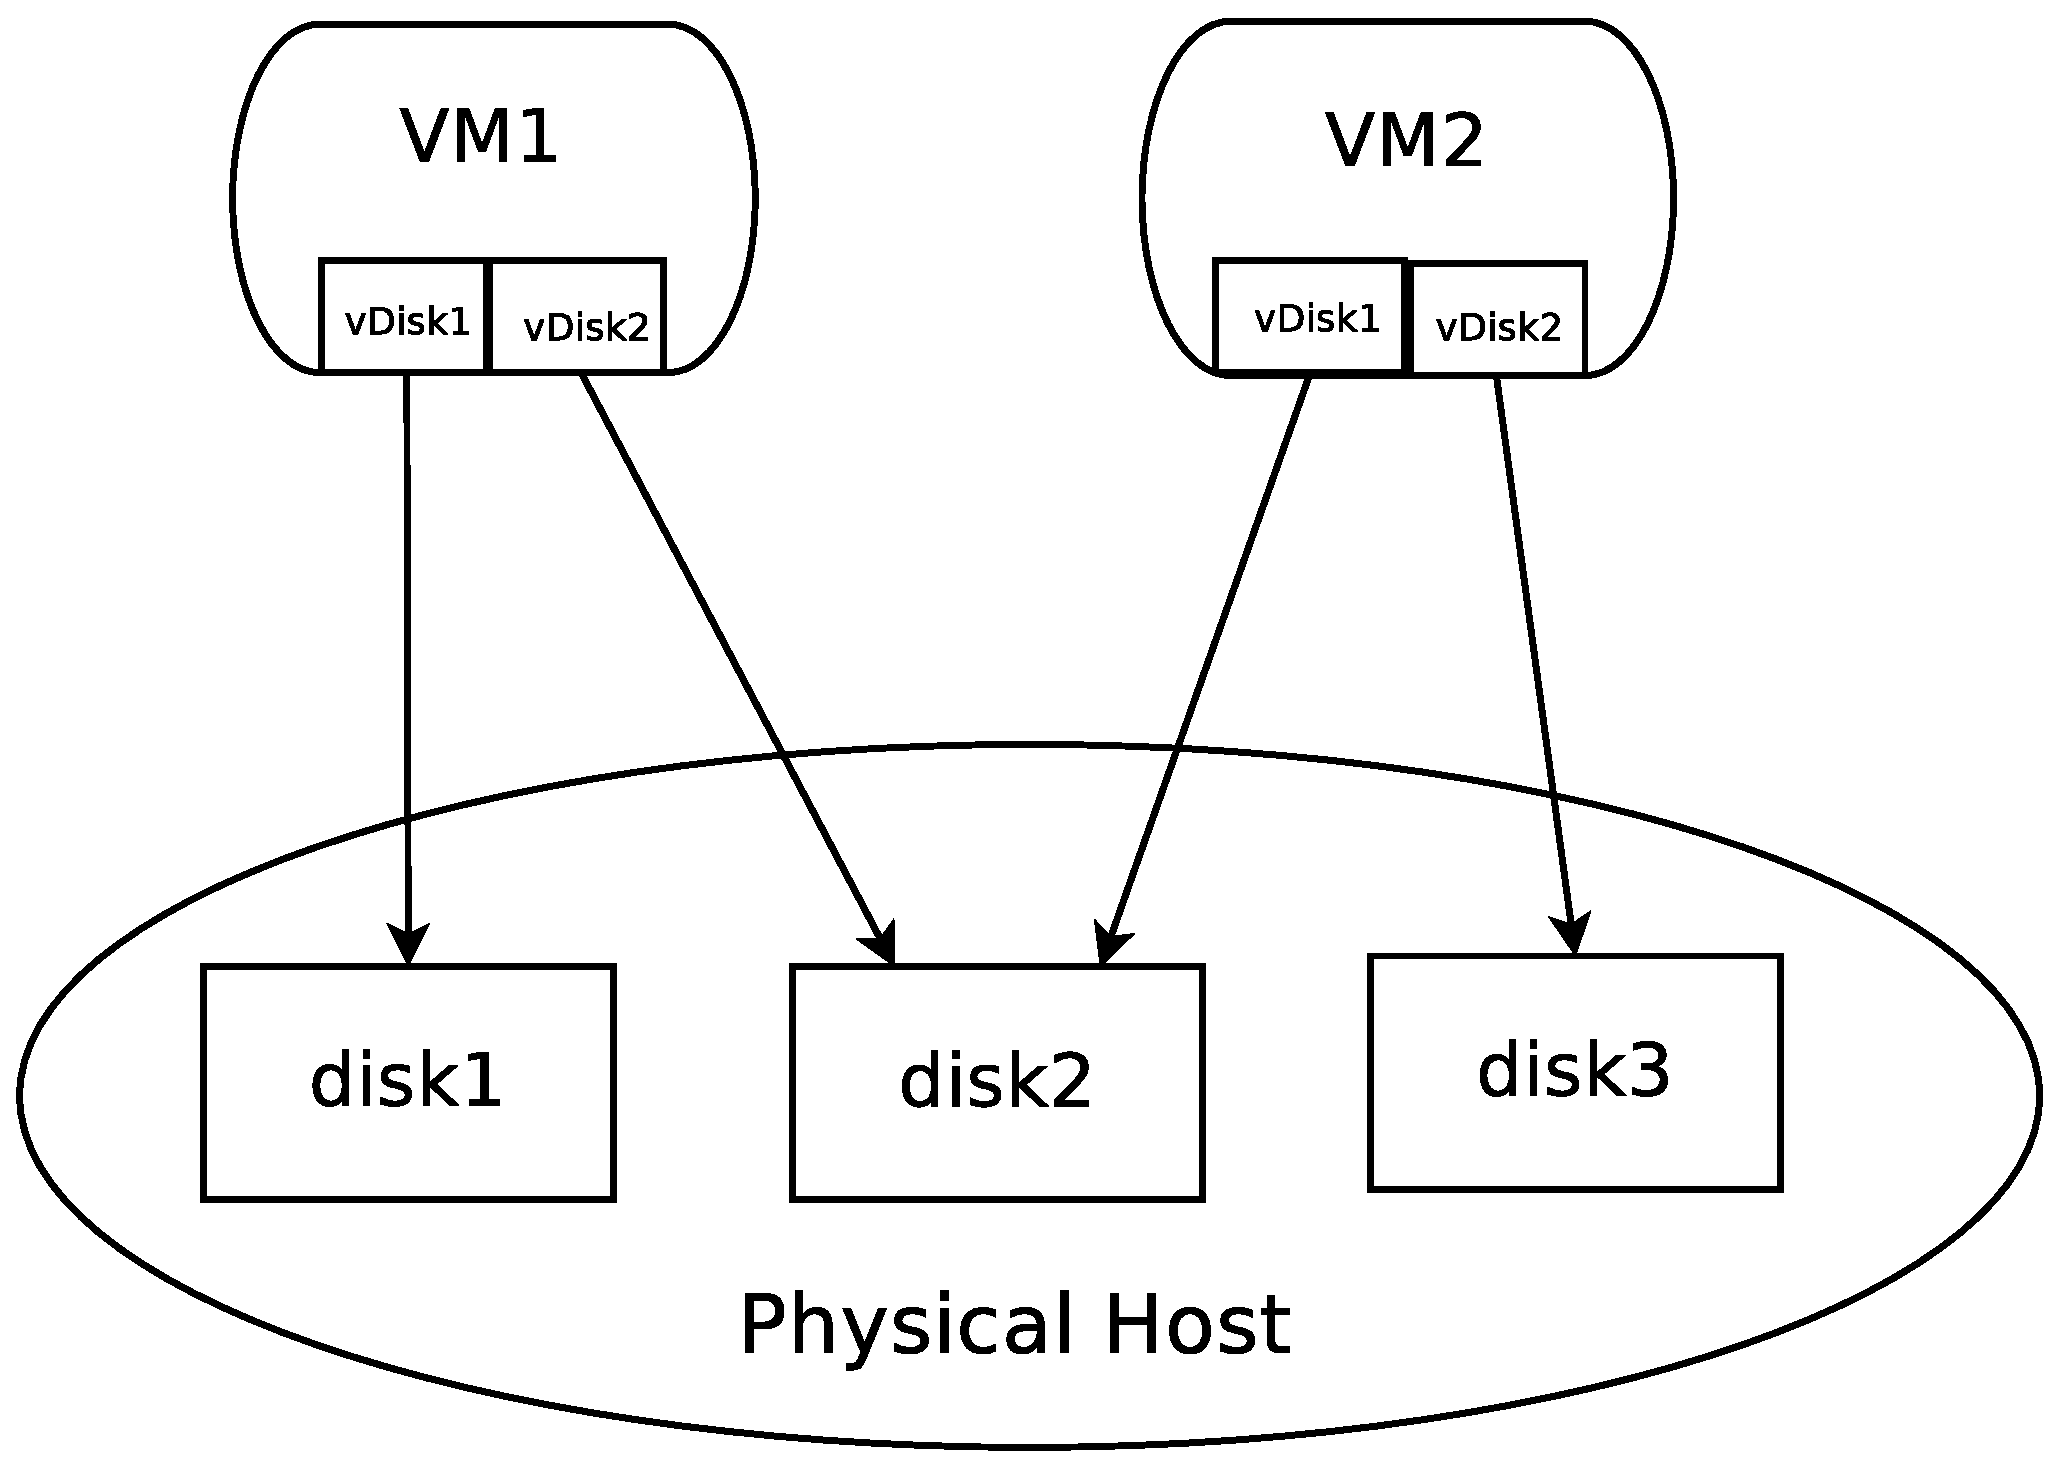
\includegraphics[width=0.5\textwidth]{figure/map}
\caption{A map example}
\label{fig:map}
\end{figure}

To overcome this limitation, in this article, we propose a solution: let 
JobTracker be aware of and maintain each TaskTracker's disk topology,  this 
algorithm can be summized as 3 steps:

\subsection{\textbf {Step 1: Let Hadoop cluster be aware of disk mapping topology}}

\begin{itemize}

\item Each slave VMs collect its disk topology which maps its virtual 
  disks to physical disks. Take table ~\ref{table:origindata} as an example, 
  $VM_1$ and $VM_2$ are hosted on physical Host 1, $VM_3$ and $VM_4$ are hosted on physical 
  host 2. The virutal disks to physical disks mapping relationship is illustrated.

\begin{table}
\centering
\caption{Virtual Disks to Physical Disks mapping topology}
\begin{tabular}{|c|c|c|}
\hline
\multirow{3}{*}{\textbf{pHost1}} &  \textbf{$VM_1$} & \textbf{$VM_2$} \\
\cline{2-3}
                        & $vDisk_{11} \mapsto pHost1:pDisk1$ & $vDisk_{21} \mapsto pHost1:pDisk2$ \\
                        & $vDisk_{12} \mapsto pHost1:pDisk2$ & $vDisk_{22} \mapsto pHost1:pDisk3$ \\
\hline
\multirow{4}{*}{\textbf{pHost2}} & \textbf{$VM_3$} & \textbf{$VM_4$} \\
\cline{2-3}
                        & $vDisk_{31} \mapsto pHost2:pDisk1$ & $vDisk_{41} \mapsto pHost2:pDisk1$ \\
                        & $vDisk_{32} \mapsto pHost2:pDisk2$ & \\
                        & $vDisk_{33} \mapsto pHost2:pDisk3$ & \\
\hline
\end{tabular}
\label{table:origindata}
\end{table}


\item When TaskTracker service launched, 
report this information to JobTracker. After JobTracker merged all topology 
info, classify overall topology based on each physical host, and send back 
related sub-topology to each VM when next heatbeat. 

Take table ~\ref{table:origindata} as example again, when this step finished, $VM_1$ and $VM_2$ 
will be aware of the sub-topology as table ~\ref{table:sub1}, $VM_3$ and $VM_4$ as table ~\ref{table:sub2}

\begin{table}[!ht]
\centering
\subfloat[sub-topology related to pHost1\label{table:sub1}]{
  \begin{tabular}{|c|}
    \hline
    Mapping Info sent to $VM_1$ \& $VM_2$ \\
    \hline
    $vDisk_{11} \mapsto pHost1:pDisk1$ \\
    $vDisk_{12} \mapsto pHost1:pDisk2$ \\
    $vDisk_{21} \mapsto pHost1:pDisk2$ \\
    $vDisk_{22} \mapsto pHost1:pDisk3$ \\
    \hline
  \end{tabular}
  \label{table:sub1}
}
\subfloat[sub-topology related to pHost2\label{table:sub2}]{
  \begin{tabular}{|c|}
    \hline
    Mapping Info sent to $VM_3$ \& $VM_4$ \\
    \hline
    $vDisk_{31} \mapsto pHost2:pDisk1$ \\
    $vDisk_{32} \mapsto pHost2:pDisk2$ \\
    $vDisk_{33} \mapsto pHost2:pDisk3$ \\
    $vDisk_{41} \mapsto pHost2:pDisk1$ \\
    \hline
  \end{tabular}
  \label{table:sub2}
}
\end{table}
\end{itemize}

\subsection{\textbf {Calculate the Disk Allocation Probability Distribution for each VM }}
\label{sec:problem1}
After step 1 finished, each VM is aware of the disk mapping topology related to the physical 
host it hosted on. 

\begin{table}
\centering
\caption{disk mapping topology}
\begin{tabular}{|c|c|c|c|c|c|}
\hline
& $pDisk_1$ & $pDisk_2$ & $pDisk_3$ & ... & $pDisk_m$ \\
\hline
$VM_1$ & $a_{11}$ & $a_{12}$ & & & \\
\hline
$VM_2$ & & $a_{22}$ & $a_{23}$ & & $a_{2m}$ \\
\hline
$VM_3$ & $a_{31}$ & $a_{32}$ & & & \\
\hline
... & & & & & \\
\hline
$VM_n$ & $a_{n1}$ & & $a_{n3}$ & & $a_{nm}$ \\
\hline
\end{tabular}
\label{table:topology}
\end{table}

Take table ~\ref{table:topology} as example, in this case, $[VM_1,VM_2,...,VM_n]$ are hosted 
on a physical host which contains $m$ physical disks($pDisk_1,pDisk_2,...,pDisk_m$), 
$a_{ij}$ is the $VM_{i}$' allocation probability for its virtual disk which mapped $pDisk_j$.

Our target is to balance I/O load on all physical disks, this can be descriped as 
an optimization issue called convex cost with linear constraints:
\begin{equation}
\begin{split}
  min\ &\sum_{j=1}^{m} (\sum_{i=1}^{n} a_{ij} - \frac{n}{m})^2 \\
  subject\ to\ &\sum_{j=1}^{m} a_{ij} = 1,\ \forall i  \\
           &a_{ij} = 0,\ \forall (i,j) \notin \Omega \\
           &0 \leq a_{ij} \leq 1,\ \forall (i,j) \in \Omega
\end{split}
\label{equ:convex}
\end{equation}

Here, $\Omega$ is defined as the union of VMs and physical disks pairs.

Let $M_{i}$ be the number of physical disks $VM_{i}$ occupies.
In this article we provide a iterative 
algorithm ~\ref{alg:iteration1} to calculate 
the approximations of the root of this equation ~\ref{equ:convex}.

\begin{algorithm}[H]
%\SetAlgoLined
\KwData{disk mapping topology of a given VM}
\KwResult{the allocation probability distribution of each virtual disk}
initialization: let $K=100, \epsilon=10^{-3}$\;
\lForEach{$i \in (1,n)$}{\
  $a_{ij_1}=a_{ij_2}=...=a_{ij_{M_i}}=\frac{1}{M_i}$ \;
}
\For{$t\leftarrow 0$ \KwTo $K$}{
  $done = 1$\;
  \lForEach{$j \in [1,m]$}{\
    $S_j=\sum_{i=1}^{n} a_{ij}$\;
  }
  \lForEach{$j \in [1,m]$}{\
    \eIf{$|S_j - \frac{n}{m}| > \epsilon$}{
      $done = 0$\;
      break\;
    }{
      continue\;
    }
  }
  \eIf{$done == 1$}{
    return matrix $\mathbf a$;
  }{
    \emph{adjust probability values to approximate optimal values}\;
    \lForEach{$a_{ij}, i \in (1,n), j \in (1,m)$}{\
      $a_{ij} = a_{ij} * \frac{n}{mS_j}$\;
    }
    \lForEach{$i, i \in (1,n)$}{\
      $T_i=\sum_{j=1}^{m} a_{ij}$\;
    }
    \lForEach{$a_{ij}, i \in (1,n), j \in (1,m)$}{\
      $a_{ij} = \frac{a_{ij}}{T_i}$\;
    }
  }
}
\caption{calculate disk allocation probability distribution}
\label{alg:iteration1}
\end{algorithm}

\subsection{\textbf {Determine disk allocation order based on probability distribution}}
\label{sec:problem2}

Given a VM and its steady-state allocation probability for each virtual disk
$\mathbf{A} = [a_1,a_2,...,a_n]$, where $N$ is $\mathbf A$'s virutual disks 
number. For each incoming creating file request, to determine which virtual disk it 
should assign, we tend to customize a $n \times n$ transition probability matrix $\mathbf {P}_A$ to 
caculate probability distribution.

Assume the probability distribution for last request is 
\begin{equation}
\mathbf{A}^{k} = [a_1^k,a_2^k,...,a_n^k]
\end{equation}
then 
\begin{equation}
\mathbf{A}^{k+1} = \mathbf{A}^{k} \mathbf{P}_A
\end{equation}

For matrix $\mathbf{P}_A$, we need to customize it to get better performance, our target is:
\begin{itemize}
  \item If $vDisk_k$ is assigned for the last request, current request should \textbf{NOT} be assigned $vDisk_k$.
  \item Beside balance disks in long-term, we should also balance them in short-term. For example, 
    given steady-state disks allocation probability $\mathbf{A} = [0.1,0.2,0.3,0.4]$, 
    even if we only request 10 times, the allocation sequence 
    determined by our algorithm should also approximate to $\mathbf{A}$.
\end{itemize}

For target 1, only need to set $p_{ii}=0,\ \forall i \in [1,n]$.

To achieve target 2, let steplength $d_{k,k+1} = |(index_{k+1} - index_{k})\ mod \ n|$, 
where $index_{k}$ defined as the assgined disk's index inside VM's virutal disks array for 
the $k$th request. We tend to minimize the average value of collection $[d_{0,1},d_{1,2},...,d_{k,k+1}]$.
By doing this, our algorithm will tend to select virtual disk one by one to guarantee 
the disk balance even in worst case or for limited times of request, similar to Round-Robin 
algorithm whose steplength equals 1.

Then, for transition probability matrix
\begin{equation}
  \mathbf{P}_A = 
  \begin{pmatrix}
    0 & p_{1,2} & p_{1,3} & \cdots & p_{1,n} \\
    p_{2,1} & 0 & p_{2,3} & \cdots & p_{2,n} \\
    p_{3,1} & p_{3,2} & 0 & \cdots & p_{3,n} \\
     \cdots & \cdots & \cdots & \cdots \\
    p_{n,1} & p_{n,2} & p_{n,3} & \cdots & 0
  \end{pmatrix}
\end{equation}

If virtual disk $i$ is selected last time, this time virtual disk $j$ will 
be selected by probability $p_{ij}$.

To minimize average steplength, 
\begin{equation}
  \begin{split}
  & p_{ij} = 0,\ if |(j-i)\ mod \ n| > \alpha_{i}, \forall i \in [1,n] \\
  s.t. & \sum_{j} p_{i,j} = 1,\ \forall i \\
       & \mathbf{AP} = \mathbf{A}
  \end{split}
\end{equation}

Based on this equation, 
\begin{equation}
    a_{j} = \sum_{k=1}^{n} a_{k} * p_{k,j},\ \forall j
\end{equation}

To optimize the following equation:
\begin{equation}
  \begin{split}
  min\ & \beta_j, \forall j \\
  s.t\ & a_{j} = a_{j-1}*p_{j-1,j} + a_{j-2}*p_{j-2,j} + ... + a_{j-\beta}*p_{j-\beta,j}
\end{split}
\label{equ:sort}
\end{equation}

We need to realign $\mathbf{A}$ to make sure the adjacent elements' difference 
value not too much. Asending sort $\mathbf {A}$ as $\mathbf{\bar{A}} = [\bar{a_1},\bar{a_2},...,\bar{a_n}]$. 
if $n$ is odd, let $\mathbf{B} = [\bar{a_1},\bar{a_3},\bar{a_5},...,\bar{a_{N-1}},\bar{a_{N}},\bar{a_{N-2}},\bar{a_{N-4}},...,\bar{a_4},\bar{a_2}]$, 
else, $\mathbf{B} = [\bar{a_1},\bar{a_3},\bar{a_5},...,\bar{a_{N-2}},\bar{a_{N}},\bar{a_{N-1}},\bar{a_{N-3}},...,\bar{a_4},\bar{a_2}]$

Let $\mathbf{P}_B$ be the transition probability matrix for $\mathbf{B}$,
Algorithm ~\ref{alg:num} shows how to determine $\beta_j$ for each column,

\begin{algorithm}[H]
%\SetAlgoLined
  \KwData{sorted steady-state probability distribution $\mathbf{B}$}
  \KwResult{no-zero elements number $\beta_j$ for each column of $\mathbf{P}_B$}
\lForEach{$j \leftarrow 1$ \KwTo $n$}{\
  sum = 0\;
  \For{$t\leftarrow 1$ \KwTo $n$}{
    $sum += b_{i-t}$\;
    \If{$sum \geq b_{j}$}{
      $\beta_j\ =\ t$\;
      break\;
    }
  }
}
\caption{Determine no-zero elements number for each column of $\mathbf{P}_B$}
\label{alg:num}
\end{algorithm}

Next, we can calculate optimal $\widetilde{\mathbf{P}}$ under constraint: 
\begin{equation}
\begin{split}
  min & ||\mathbf{b}\widetilde{P}-\mathbf{b}||_{2} \\
 s.t. & \sum_{j=1}^{m} p_{ij}=1, \forall i \\
      & p_{ij} = 0, \forall (i,j) \notin \Omega_{\widetilde{P}} \\
      & 0 \leq p_{ij} \leq 1, \forall (i,j) \in \Omega_{\widetilde{P}}
\end{split}
\end{equation}

Here we provide a interative algorithm ~\ref{alg:num}:

\begin{algorithm}[H]
  \KwData{$\mathbf{B}$ and $\beta_j,\forall j$}
  \KwResult{Transition probability matrix $\mathbf{P}_B$}
  initialization: let $K=1000, \epsilon=10^{-3}$\;
  \For{$t \leftarrow 1$ \KwTo $K$}{\
    \For{$i \leftarrow 1$ \KwTo $n$}{\
      count number of no-zero elements number $M$ based on all $\beta_j$\;
      \lForEach{$j$}{
        $p_{ij} = \frac{1}{M}$\;
      }
    }
    calculate $\hat{\mathbf{B}} = \mathbf{BP_B}$\;
    \If{$\sum_i {(\hat{b_i}-b_i)^2} < \epsilon$}{
      return $\mathbf{B}$\;
    }
    \lForEach{$i$}{
      $c_i=\frac{\hat{b_i}}{b_i}$\;
    }
    \lForEach{$i,j$}{
      $p_{ij} = \frac{p_{ij}}{c_i}$
    }
  }
  \caption{Determine no-zero elements number for each column of $\mathbf{P}_B$}
  \label{alg:num}
\end{algorithm}

In some worst cases, algorithm ~\ref{alg:num} may not be able to convergent to 
the $\epsilon$, to solve it, a greedy stragety is designed as algorithm ~\ref{alg:greedy}

Finally, let $e_i=(0,0,...,1,0,...,0)^{T}$, where the i element equals 1, all 
others equal 0, then the disk allocation for each creating file request can 
be described as algorithm ~\ref{alg:final}

\begin{algorithm}[H]
\While{True}{\
  run algorithm ~\ref{alg:num}\;
  \If{cannot achieve $\sum_i {(\hat{b_i}-b_i)^2} < \epsilon$}{\
    save $\widetilde{\mathbf{P_B}}$\;
    find $k_{min} = \{k|\beta_j[k^{'}] > \beta_j[k_{min}], \forall k^{'}\}$\;
    \eIf{$\beta_j[k_{min}] == length\ of\ B$}{
      break
    }{
      $\beta_j[k_{min}] += 1$\;
      re-initialize $\mathbf{P_B}$ based on new $\beta_j$\;
      $\mathbf{P_B} = 0.5 * (\mathbf{P_B} + \widetilde{\mathbf{P_B}})$
    }
  }
}
\caption{Greedy algorithm to improve algorithm ~\ref{alg:num} }
\label{alg:greedy}
\end{algorithm}


\begin{algorithm}[H]
  \KwData{steady-state probability distrubution $\mathbf{B}$}
  initialization: $\alpha=random(n)$, $\pi_{1} = e_{\alpha}$\;
  calculate transition probability matrix $\mathbf{P}$ based;
  \lForEach{$k$th request from client, $k > 1$}{\
    $\pi_{k} = \pi_{k-1} \mathbf{P}$\;
    select disk based on the prabability $\pi_{k}$;
  }
\caption{Algorithm 1}
\label{alg:final}
\end{algorithm}

Based on this algorithm, we can guarantee the actual disk selection sequence 
approximate to the steady-state probability distribution, even in worst case or for limited times of request. If all the probability 
values of the steady-state distribution are the same, this algorithm 
equivalent to Round-Robin algorithm.

\section{\textbf\normalsize{EXPERIMENT}}
To demonstrate the feasilibity of this algorithm, a simulation program is implemented 
as\\
\textbf{git@github.com:xiaodingbian/disk-allocation.git}.
In this repository, log file "result\_20\_40.log" is a running result with 20 VMs and 40 physical disks.
And cos similarity function is used to evaluate whether generated sequence for a few requests can 
follow to steady-state probability distribution.

\end{document}

